%%%%%%%%%%%%%%%%%%%%%%%%%%%%%%%%%%%%%%%%%%%%%%%%%%%%%%%%
\documentclass[10pt, aspectratio=169]{beamer}
\usepackage[many]{tcolorbox}
\usetheme{metropolis}
\usepackage[english]{babel}
\usepackage[utf8]{inputenc}
\usepackage[T1]{fontenc}
\usepackage{array}
\usepackage{booktabs}
\usepackage{colortbl}
\usepackage{multirow}
\usepackage{graphicx}
\usepackage{mathrsfs}
\usepackage{bbding}
\usepackage{pifont}
\usepackage{wasysym}
\usepackage{amssymb}
\usepackage{enumerate}
\usepackage{booktabs,threeparttable}
\usepackage{adjustbox}
\usepackage{tikz}
\usetikzlibrary{calc}
\usepackage{geometry}
\usepackage{appendixnumberbeamer}


% DEFINE COLORPALETTE
\newcommand{\cmark}{\ding{51}}%
\newcommand{\xmark}{\ding{55}}
\definecolor{unibasmintlight}{RGB}{233, 255, 253}
\definecolor{unibasmint}{RGB}{165,215,210}
\definecolor{unibasmintmid}{RGB}{30,165,165}
\definecolor{unibasanthr}{RGB}{45,55,60}
\definecolor{unibasgreydark}{RGB}{140,145,150}
\definecolor{unibasred}{RGB}{210,5,55}
\definecolor{unibaspink}{RGB}{235,130,155}
\definecolor{unibasgrey}{RGB}{190,195,200}
\definecolor{unibasmintdark}{RGB}{0,110,110}
\definecolor{unibasblack}{RGB}{0,0,0}
\definecolor{unibaswhite}{RGB}{255,255,255}

\definecolor{scenA_table}{RGB}{245, 245, 180}
\definecolor{scenB_table}{RGB}{235, 215, 245}
\definecolor{scenC_table}{RGB}{200, 225, 240}

\definecolor{capacity_upgrade}{RGB}{64, 153, 153}
\definecolor{capacity_expansion}{RGB}{162, 216, 216}


% -------------------------------------------------------
% METROPOLIS COLOR SETUP
% -------------------------------------------------------
% \setbeamercolor{normal text}{fg=unibasanthr, bg=white}
% \setbeamercolor{alerted text}{fg=unibasred}
% \setbeamercolor{example text}{fg=unibasmintdark}

% \setbeamercolor{frametitle}{bg=unibasmintlight, fg=unibasmintdark}
% \setbeamercolor{title separator}{fg=unibasmintdark}
% \setbeamercolor{progress bar}{fg=unibasmintdark, bg=unibasgrey}

% \setbeamercolor{block title}{bg=unibasmintdark, fg=unibasmint}
% \setbeamercolor{block body}{bg=unibasmintlight, fg=unibasanthr}
% \setbeamercolor{block title alerted}{bg=unibasred, fg=white}
% \setbeamercolor{block body alerted}{bg=unibasmintlight!50, fg=unibasanthr}

% \setbeamercolor{title}{fg=unibasmintdark}
% \setbeamercolor{subtitle}{fg=unibasgreydark}
% \setbeamercolor{author}{fg=unibasanthr}
% \setbeamercolor{institute}{fg=unibasgreydark}
% \setbeamercolor{date}{fg=unibasgreydark}

% \setbeamercolor{section in toc}{fg=unibasmintdark}
% \setbeamercolor{subsection in toc}{fg=unibasgreydark}

% \setbeamercolor{itemize item}{fg=unibasmintdark}
% \setbeamercolor{itemize subitem}{fg=unibasmintmid}
% \setbeamercolor{itemize subsubitem}{fg=unibasgreydark}
% \setbeamercolor{enumerate item}{fg=unibasmintdark}

% \setbeamercolor{button}{bg=unibasmint, fg=unibasanthr}

% footer / standout
\setbeamercolor{footline}{fg=unibasgreydark, bg=white}

% -------------------------------------------------------
% METROPOLIS FONT / STYLE OPTIONS
% -------------------------------------------------------
\metroset{
  titleformat        = regular,
  titleformat frame  = regular,
  sectionpage        = none,
  numbering          = fraction,
  progressbar        = frametitle,
  block              = fill
}

\usefonttheme[onlymath]{serif}
\setbeamertemplate{caption}[numbered]


% % -------------------------------------------------------
% % BLOCK ENVIRONMENT COLORS (inside block/alertblock)
% % -------------------------------------------------------
% \AtBeginEnvironment{block}{%
%   \setbeamercolor{itemize item}{fg=unibasmintdark}
%   \setbeamercolor{itemize subitem}{fg=unibasmintmid}
%   \setbeamercolor{enumerate item}{fg=unibasmintdark}
%   \setbeamercolor{item projected}{fg=white, bg=unibasmintdark}
% }

% \AtBeginEnvironment{alertblock}{%
%   \setbeamercolor{itemize item}{fg=unibasred}
%   \setbeamercolor{enumerate item}{fg=unibasred}
%   \setbeamercolor{item projected}{fg=white, bg=unibasred}
% }

% -------------------------------------------------------
% CITATIONS
% -------------------------------------------------------
\usepackage[backend=biber, style=apa, maxbibnames=999, minbibnames=1,
            maxcitenames=1, mincitenames=1, uniquelist=true]{biblatex}
\addbibresource{optimalpv_conf.bib}
\AtBeginBibliography{\small}
% \hypersetup{colorlinks=true,
%             citecolor=unibasmintmid,
%             linkcolor=unibasmintdark,
%             urlcolor=unibasmintdark}

% -------------------------------------------------------
% BACKUP FRAME COUNTER
% -------------------------------------------------------
\newcommand{\backupbegin}{
  \newcounter{framenumberappendix}
  \setcounter{framenumberappendix}{\value{framenumber}}
}
\newcommand{\backupend}{
  \addtocounter{framenumberappendix}{-\value{framenumber}}
  \addtocounter{framenumber}{\value{framenumberappendix}}
}

% -------------------------------------------------------
% TITLE INFO
% -------------------------------------------------------
\title[Improved Residential PV Expansion]{Decisions at the Grid's Edge}
\subtitle{An Improved Spatial PV Expansion in Swiss Residences}
\author{Raul Hochuli}
\institute{University of Basel, Faculty of Business and Economics}
\date{June 2026}
% \titlegraphic{\includegraphics[width=2.3cm]{UniBas_Logo.jpg}}


%*******************************************************************************
\begin{document}
%*******************************************************************************

% -------------------------------------------------------
\begin{frame}
  \maketitle
\end{frame}


%%%%%%%%%%%%%%%%%%%%%%%%%%%%%%%%%%%%%%%%%%%%%%%
\section{Motivation \& Literature}

% -------------------------------------------------------
\begin{frame}{Motivation}
  \centering
  \makebox[0pt][c]{%
    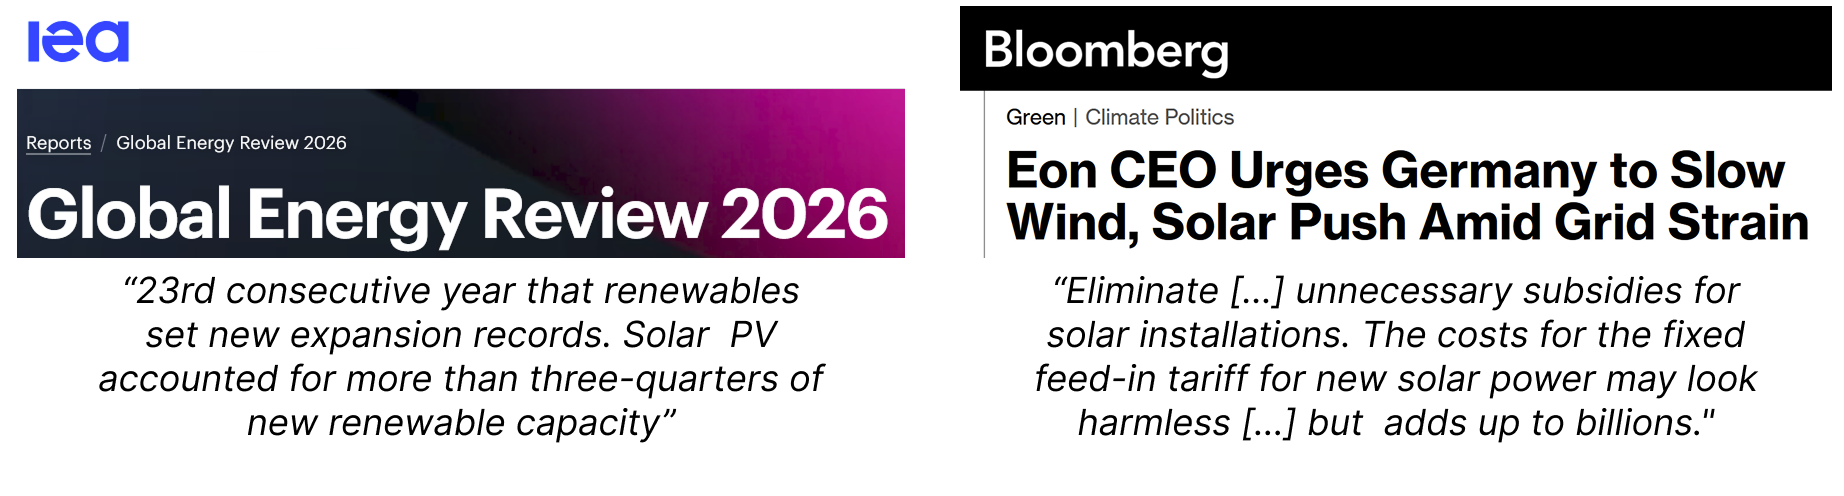
\includegraphics[width=0.9841\textwidth]{figures/newspaper_header3.png}
  }
\vspace{-0.25cm}
  \begin{block}{Research Contribution}
    \begin{enumerate}
      \item \textbf{Problem quantification} $\rightarrow$\textit{Build an extensive data based model simulation that estimates how soon and when solar PV expansion causes "grid-problems".}
      \vspace{-0.101cm}
      \item \textbf{Economic response} $\rightarrow$ \textit{2nd-best solution: Simple subsidy adjustments might delay grid congestion for a more efficient outcome.}
      \vspace{-0.101cm}
      \item \textbf{Not included} $\rightarrow$ \textit{Local battery storage is not included in the simulation, but considered in post-analysis.}
    \end{enumerate}
  \end{block}
\end{frame}

% -------------------------------------------------------
\begin{frame}{About PV}
\centering
\definecolor{card1}{RGB}{165,200,220}
\definecolor{card2}{RGB}{125,165,190}
\definecolor{card3}{RGB}{90,130,160}
\definecolor{card4}{RGB}{55,95,130}
\definecolor{card5}{RGB}{25,60,95}
\definecolor{card6}{RGB}{0,25,60}
\definecolor{bottomcard}{RGB}{45,55,60}

\pgfmathsetmacro{\dx}{2.8}   
\pgfmathsetmacro{\barleft}{-1.25}          % t1 left edge (half of 2.5cm card)
\pgfmathsetmacro{\barright}{4.1*\dx + 1.2} % s2 right edge
\pgfmathsetmacro{\barwidth}{(\barright - \barleft)}
\pgfmathsetmacro{\barcenter}{(\barleft + \barright)/2}


\begin{tikzpicture}[xscale=0.96, yscale=0.96, transform shape, xshift=-0.8cm]
\newcommand{\cardwidth}{2.0cm}
\tikzset{
  topiccard/.style={
    rounded corners=6pt,
    minimum width=2.5cm,
    minimum height=3.3cm,
    align=left,
    text=white,
    font=\small
  },
  smallcard/.style={
    rounded corners=6pt,
    minimum width=2.4cm,
    minimum height=0.9cm,
    align=left,
    text=white,
    font=\small
  }
}

% MAIN ROW
\node[topiccard, fill=card3, fill opacity = 0.25, text opacity = 0.95] (t1) at (0*\dx, 0)
% \node[topiccard, fill=card3] (t1) at (0*\dx, 0)
{
\begin{minipage}{\cardwidth}
\raggedright
{\bfseries Goals \& Scenarios}\\
\vspace{0.1cm}
\scriptsize
37.5 GW by 2050 \hyperlink{appendix_res_targets}{\beamerreturnbutton{\tiny{Targets}}}\\
\hfill{\tiny\cite{bfe_ep2050_2020}}
\end{minipage}
};

\node[topiccard, fill=card4, fill opacity = 0.25, text opacity = 0.95] (t2) at (1*\dx, 0)
{
\begin{minipage}{\cardwidth}
\raggedright
{\bfseries Grid Cost Estimates}\\
\vspace{0.1cm}
\scriptsize
LV: CHF 600m pa until 2050\\
\hfill{\tiny\cite{bfe_ep2050_netz2022}}\\
\vspace{0.05cm}
Poss. underestimation \hyperlink{appendix_model_grid_analysis}{\beamerreturnbutton{\tiny{Grid Analysis}}}
\end{minipage}
};

\node[topiccard, fill=card5, fill opacity = 0.25, text opacity = 0.95] (t3) at (2*\dx, 0)
{
\begin{minipage}{\cardwidth}
\raggedright
{\bfseries Drivers \& Acceptance}\\
\vspace{0.1cm}
\scriptsize
Key Factors\\
\hfill{\tiny\cite{muller2020}}\\
\vspace{0.05cm}
Reluctance\\
\hfill{\tiny\cite{sutterlin2017, cousse2020}}
\end{minipage}
};

\node[topiccard, fill=card6] (t4) at (3*\dx, 0)
{
\begin{minipage}{\cardwidth}
\raggedright
{\bfseries Future / Optimal Inst.}\\
\vspace{0.1cm}
\scriptsize
NPV Proxy\\
\hfill{\tiny\cite{arguello2018}}\\
\vspace{0.05cm}
MV grid\\
\hfill{\tiny\cite{gupta2021}}\\
\vspace{0.05cm}
Biodiversity a.o.\\
\hfill{\tiny\cite{hermoso2023}}
\end{minipage}
};

% STACKED PAIR
\node[smallcard, fill=card2, fill opacity = 0.25, text opacity = 0.95] (s1) at (4.1*\dx, 0.801)
{
\begin{minipage}{\cardwidth}
\raggedright
{\bfseries Grid Effects}\\
\vspace{0.05cm}
\scriptsize
Penetration limits\\
\hfill{\tiny\cite{tevar2019}}
\end{minipage}
};

\node[smallcard, fill=card2, fill opacity = 0.25, text opacity = 0.95] (s2) at (4.1*\dx, -0.801)
{
\begin{minipage}{\cardwidth}
\raggedright
{\bfseries Smart Meters}\\
\vspace{0.05cm}
\scriptsize
Rollout 2028 at 80\%\\
\hfill{\tiny\cite{elcom_smartmeter_2026}}
\end{minipage}
};

% BOTTOM SUMMARY CARD
\node[
  rounded corners=8pt,
  fill=bottomcard,
  minimum width=\barwidth cm,
  minimum height=0.65cm,
  text=white,
  align=center
] (bottom) at (\barcenter, -2.15)
{
  \small Increasing PV deployment outpaces grid infrastructure (globally).
};

% CONNECTION LINES
\foreach \n in {t1,t2,t3,t4}
{
  \draw[gray!60, thick]
  (\n.south) -- (\n.south |- bottom.north);
}

\draw[gray!60, thick]
  (s2.south) -- (s2.south |- bottom.north);

\end{tikzpicture}

\vspace{0.01cm}
\makebox[0pt][c]{%
  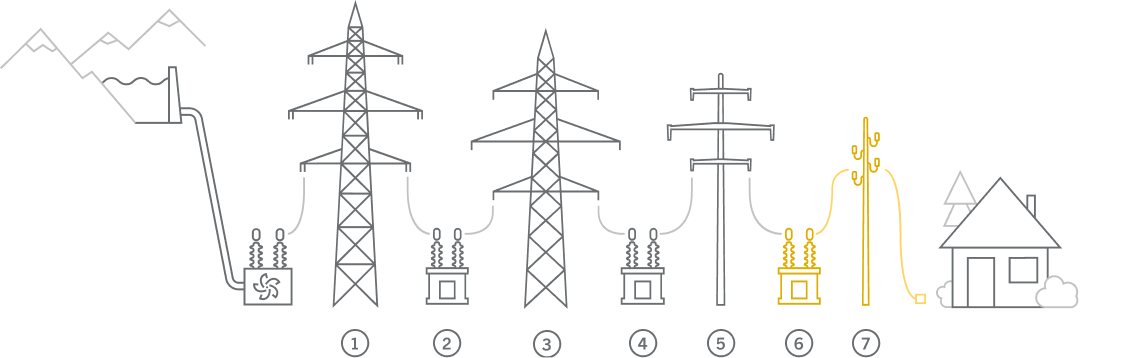
\includegraphics[width=0.751\textwidth]{figures/grid-levels.png}
}
\end{frame}


%%%%%%%%%%%%%%%%%%%%%%%%%%%%%%%%%%%%%%%%%%%%%%%
\section{Model}

% -------------------------------------------------------
\begin{frame}{Model Simulation - 3 Agents}
\hypertarget{mod_structure_agents}{}

\begin{columns}[t]

\begin{column}{0.49\textwidth}
  \only<1->{\textcolor[RGB]{128,0,128}{Production}
  \vspace{-0.0961cm}
  \begin{itemize}
    \item Roof partitions and radiation time series yield production potential.
    \vspace{-0.0961cm} 
    \item Calibrated random forest assigns installation size \hyperlink{appendix_randomforest_scatterplot}{\beamerreturnbutton{App. RFR}}.
  \end{itemize}}
  \only<2->{\textcolor[RGB]{204,85,0}{Demand} ($\rightarrow$ \textcolor[RGB]{0,70,127}{Feed-in})
  \vspace{-0.0961cm}
  \begin{itemize}
    \item 6 Archetype profiles scaled by living area (\cite{swissstore2022}).
    \vspace{-0.0961cm}
    \item Heat pumps: Scaling up winter months.
  \end{itemize}}
  \only<3->{\textcolor{unibasgreydark}{Investments}
  \vspace{-0.0961cm}
  \begin{itemize}
    \item General cost assumption of PV calculator (\cite{energieschweiz2023} \hyperlink{appendix_cost_function}{\beamerreturnbutton{App. Cost}})
  \end{itemize}
  % $\rightarrow NPV_{i} = -Inv_{i} + \sum_{t}^{25}\frac{SelfCons_{i,t} P_{elec,t} + Feedin_{i,t} P_{pv,t}}{(1+r)^t}$}
  }
  \vspace{0.35cm}
  \only<4->{$\rightarrow NPV_{i} = -Inv_{i} + \sum_{t}^{25}\frac{SelfCons_{i,t} + Feedin_{i,t} }{(1+r)^t}$
  }
  \vfill
\end{column}

\begin{column}{0.49\textwidth}
  \begin{figure}
    \centering
    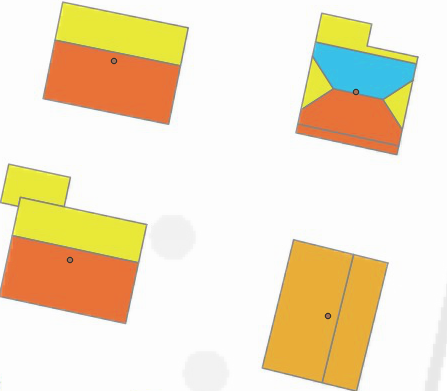
\includegraphics[width=0.481\linewidth]{figures/EGID_solkat_example.png}
  \end{figure}
  \vspace{-0.2cm}
  \begin{figure}
    \centering
    \only<1>{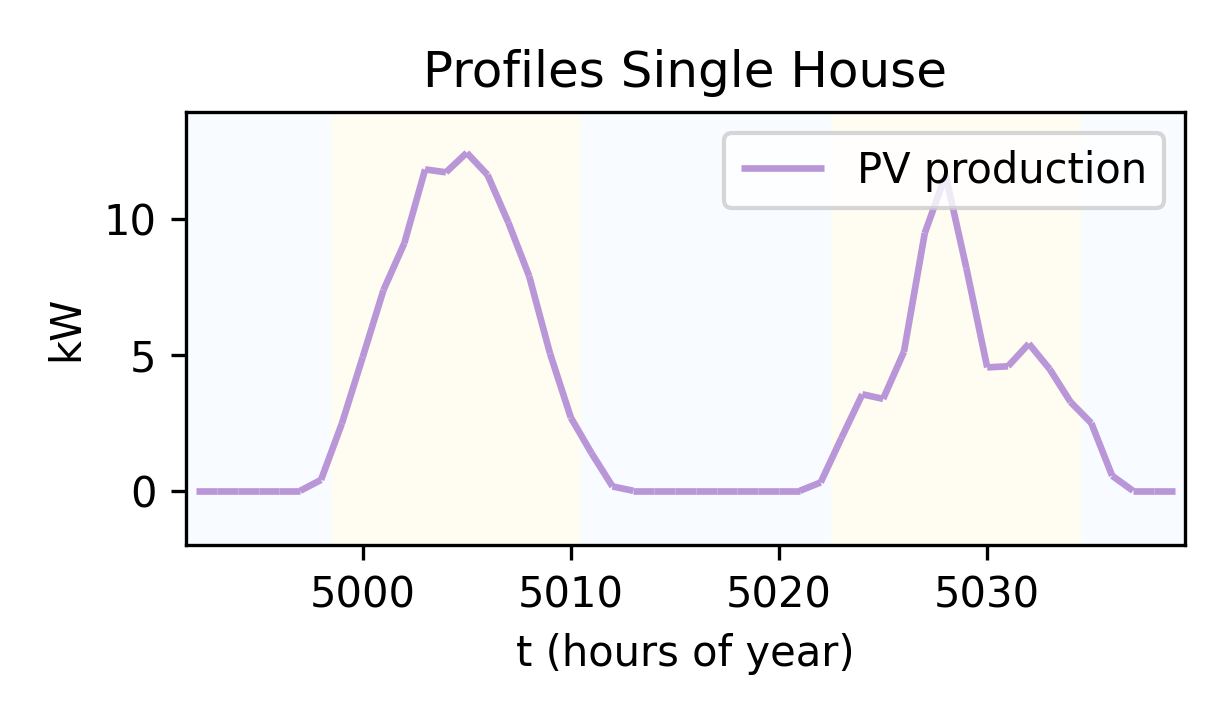
\includegraphics[width=0.91\linewidth]{figures/plot_EGID_HOY_pvprod.png}}%
    \only<2>{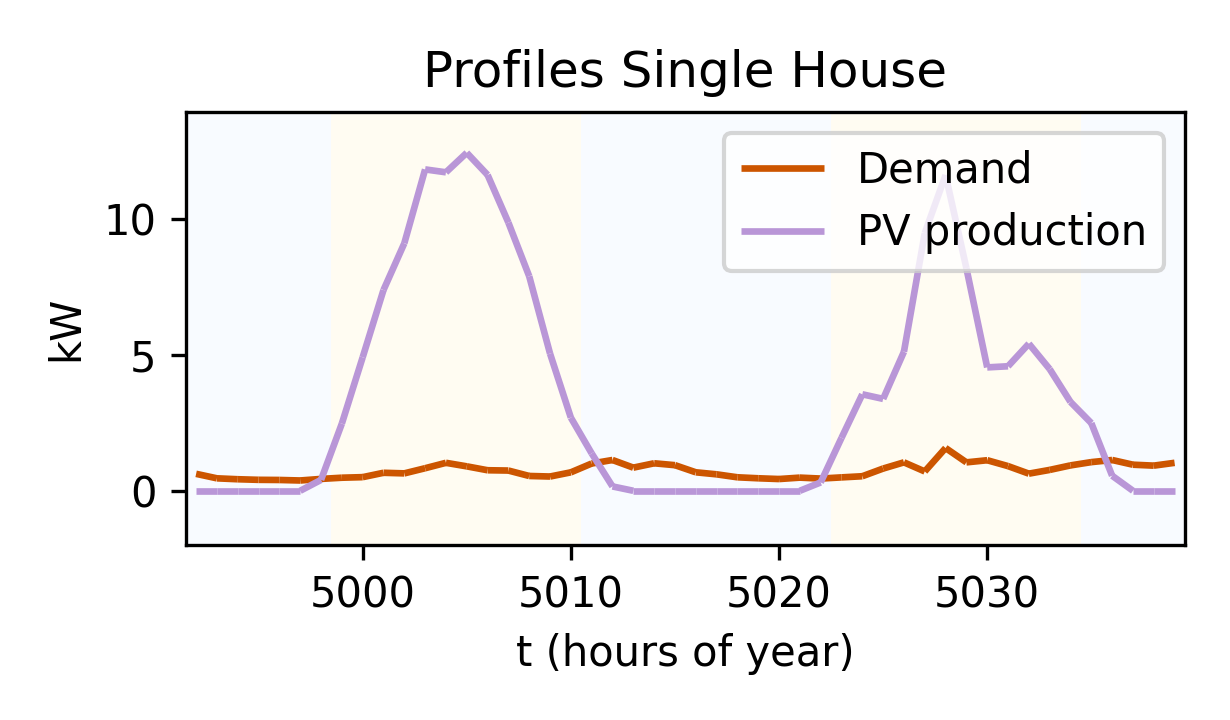
\includegraphics[width=0.91\linewidth]{figures/plot_EGID_HOY_pvprod_demand.png}}%
    \only<3->{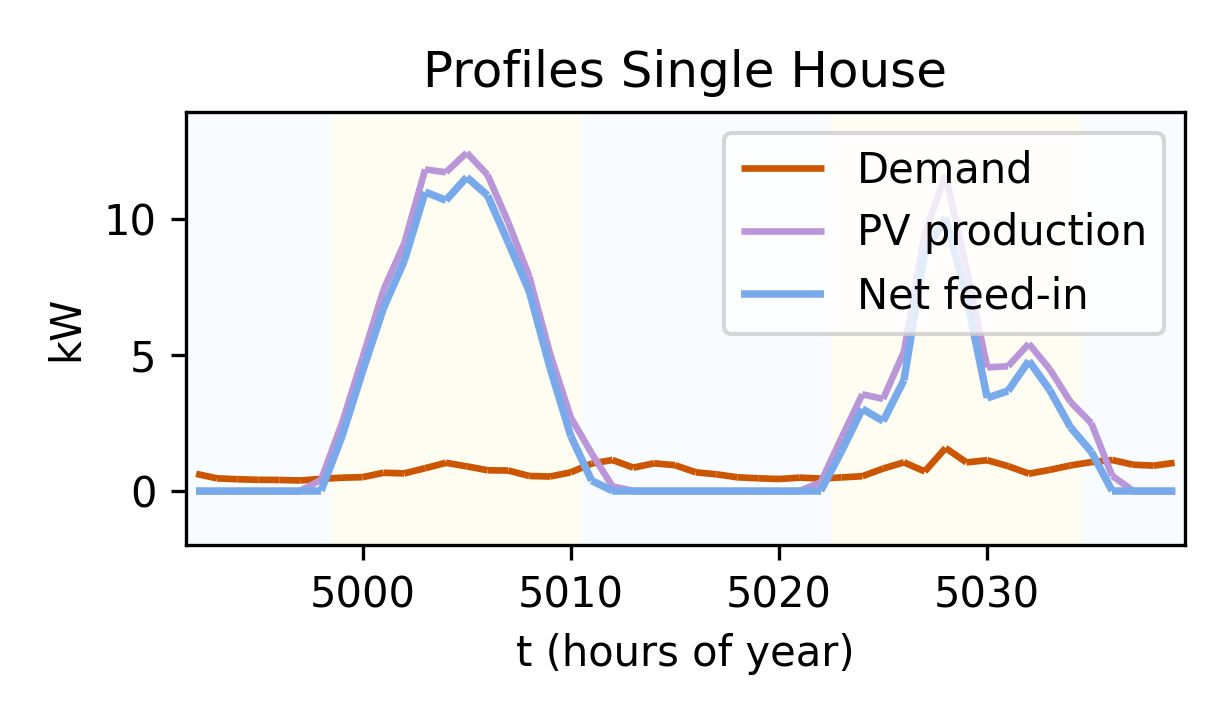
\includegraphics[width=0.91\linewidth]{figures/plot_EGID_HOY_pvprod_demand_feedin.png}}%
  \end{figure}
\end{column}

\end{columns}
\end{frame}

% -------------------------------------------------------
\begin{frame}{Allocation Process}
\hypertarget{mod_allocation_process}{}

\begin{columns}[t]

\begin{column}{0.49\textwidth}
  \textbf{Allocation process}
  \begin{itemize}
    \item NPV defines installation "order" (similar to \cite{arguello2018},
      \hyperlink{appendix_npv_hist_sensitivity}{\beamerreturnbutton{App. NPV}}).
    \item Scaled, adjusted, annual ``construction budget'' (\cite{bfe_ep2050_2020}) until 2050.
  \end{itemize}

  \vspace{-0.2cm}
  \begin{figure}
    \centering
    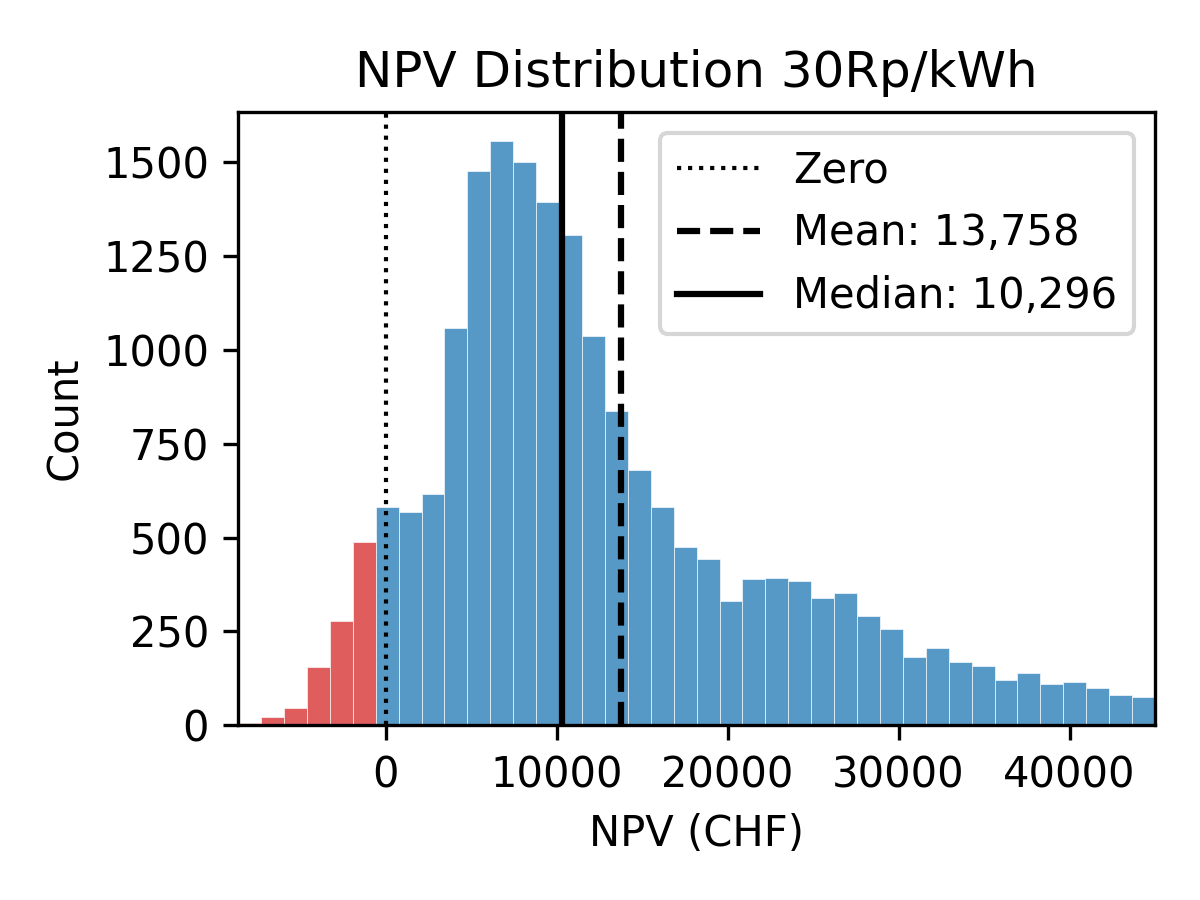
\includegraphics[width=0.84\linewidth]{figures/NPVhist_LRG3_max.png}
  \end{figure}
\end{column}

\begin{column}{0.49\textwidth}
  \textbf{Subsidy adjustment}
  \begin{itemize}
    \item Subsidy budget given to operator (transparent criteria)
    \item 3 types (A: roof orientation, B: grid specific, C: combination)
  \end{itemize}

  \[
    \rightarrow NPV_{i,X} = NPV_{i} + S_{i,X} - R_{i,X}
  \]

  \vspace{0.3cm}
  \centering
  \footnotesize
  \begin{tabular}{|l| c c c c|}
    \hline
    & $S=0$ & 4000 & 6000 & 8000 \\
    \hline
    $R=0$ & BU & \cellcolor{scenA_table} & \cellcolor{scenA_table} A & \cellcolor{scenA_table} \\
    4000  & \cellcolor{scenB_table} & \cellcolor{scenC_table} & \cellcolor{scenC_table} & \cellcolor{scenC_table} \\
    6000  & \cellcolor{scenB_table} B & \cellcolor{scenC_table} & \cellcolor{scenC_table} C & \cellcolor{scenC_table} \\
    8000  & \cellcolor{scenB_table} & \cellcolor{scenC_table} & \cellcolor{scenC_table} & \cellcolor{scenC_table} \\
    \hline
  \end{tabular}
\end{column}

\end{columns}
\end{frame}


%%%%%%%%%%%%%%%%%%%%%%%%%%%%%%%%%%%%%%%%%%%%%%%
\section{Data}

% -------------------------------------------------------
\begin{frame}{Data}

\begin{columns}[t]
\begin{column}{0.48\textwidth}

  \centering\textbf{Summary}\\
  \vspace{0.2cm}
  {\scriptsize
  \setlength{\tabcolsep}{3.5pt}
  \renewcommand{\arraystretch}{1.15}
  \begin{tabular}{l c c c}
    \hline
    \textbf{Parameter} & \textbf{Sample} & \textbf{Avail.} & \textbf{All CH} \\
    \hline
    n Municipalities         & 28     & 79      & 2'133     \\
    n All Buildings          & 44'354 & 132'018 & 3'090'962 \\
    n Resid. Houses          & 21'599 & 47'900  & 1'716'194 \\
    n Grid Nodes             & 391    & 1'113   & --        \\
    Inst. Cap. 2024 (MW)     & 20.6   & 79.0    & 2'450.1   \\
    Capacity 2050 (MW)       & 115.6  & 739.5   & 17'313.8  \\
    \hline
  \end{tabular}
  }

\end{column}
\begin{column}{0.48\textwidth}

  \centering\textbf{Data Sources}\\
  \vspace{0.2cm}
  {\scriptsize
  \setlength{\tabcolsep}{3.5pt}
  \renewcommand{\arraystretch}{1.15}
  \begin{tabular}{l l l}
    \hline
    \textbf{Category} & \textbf{Description} & \textbf{Ref.} \\
    \hline
    Rooftop Data      & Roof surface, orientation, tilt             & [1]     \\
    Building Data     & Type, heating, prices/tariffs               & [2--5]  \\
    Grid Infra.       & Nodes, connections + capacity               & (NDA)   \\
    Other Data        & Demand, costs, targets, radiation           & [6--9]  \\
    Computing         & HPC cluster for model run                   & [10]    \\
    \hline
  \end{tabular}
  \vspace{0.2cm}
  }

  {\tiny
  \raggedright
  [1]: \cite{solkat2023}\par
  [2--5]: \cite{gwr2025, elec_prod2024, vese_pvtarif2023, elcom2023}\par
  [6--9]: \cite{swissstore2022, energieschweiz2023, bfe_ep2050_2020, meteoblue2023}\par
  [10]: \cite{hpc_scicore2026}\par
  }

\end{column}
\end{columns}
\end{frame}


%%%%%%%%%%%%%%%%%%%%%%%%%%%%%%%%%%%%%%%%%%%%%%%
\section{Results}

% -------------------------------------------------------
\begin{frame}{PV-Induced Excess Feed-in}
\begin{minipage}{0.322\textwidth}
  \centering
\includegraphics[width=\textwidth]{figures/gridnode_feedin_threshold_HOY.png}
\end{minipage}\hfill
\begin{minipage}{0.322\textwidth}
  \centering
\includegraphics[width=\textwidth]{figures/line_PVproduction_bau_excfeedin.png}
\end{minipage}\hfill
\begin{minipage}{0.322\textwidth}
  \centering
\includegraphics[width=\textwidth]{figures/line_PVproduction_bau_feedin.png}
\end{minipage}
\end{frame}

% -------------------------------------------------------
\begin{frame}{Different Subsidies}
\begin{minipage}{0.48\textwidth}
  \centering
\includegraphics[width=\textwidth]{figures/line_PVproduction_bauABC_excfeedin.png}
\end{minipage}\hfill
\begin{minipage}{0.48\textwidth}
  \centering
\includegraphics[width=\textwidth]{figures/line_PVproduction_bauABC_feedin.png}
\end{minipage}
\end{frame}

% -------------------------------------------------------
\begin{frame}{Grid Optimal Expansion}
\begin{minipage}{0.48\textwidth}
  \centering
\includegraphics[width=\textwidth]{figures/line_PVproduction_gridoptim_excfeedin.png}
\end{minipage}\hfill
\begin{minipage}{0.48\textwidth}
  \centering
\includegraphics[width=\textwidth]{figures/line_PVproduction_gridoptim_feedin.png}
\end{minipage}
\end{frame}


% -------------------------------------------------------
\begin{frame}{Worst Week in Worst Node}
\begin{minipage}{0.48\textwidth}
  \centering
  \vspace{0.3cm}
  {\small
  \begin{tabular}{ll}
    \toprule
    \textbf{Parameter} & \textbf{Value} \\
    \midrule
    % Worst node                       & 751 \\
    Peak day 1                          & 2025-07-12 to 2025-07-13 \\
    Peak day 1 end                       & 2025-07-13 \\
    Total excess feed-in                & 5'970.7 kWh \\
    n Houses                            & 379 \\
    Avg.\ excess feed-in p.\ house      & 15.8 kWh \\
    Tesla Powerwall (\cite{tesla2026})  & 13.5 kWh\\
    Avg.\ demand p.\ house              & 3.0  kWh\\
    \bottomrule
  \end{tabular}
  }
\end{minipage}\hfill
\begin{minipage}{0.48\textwidth}
  \centering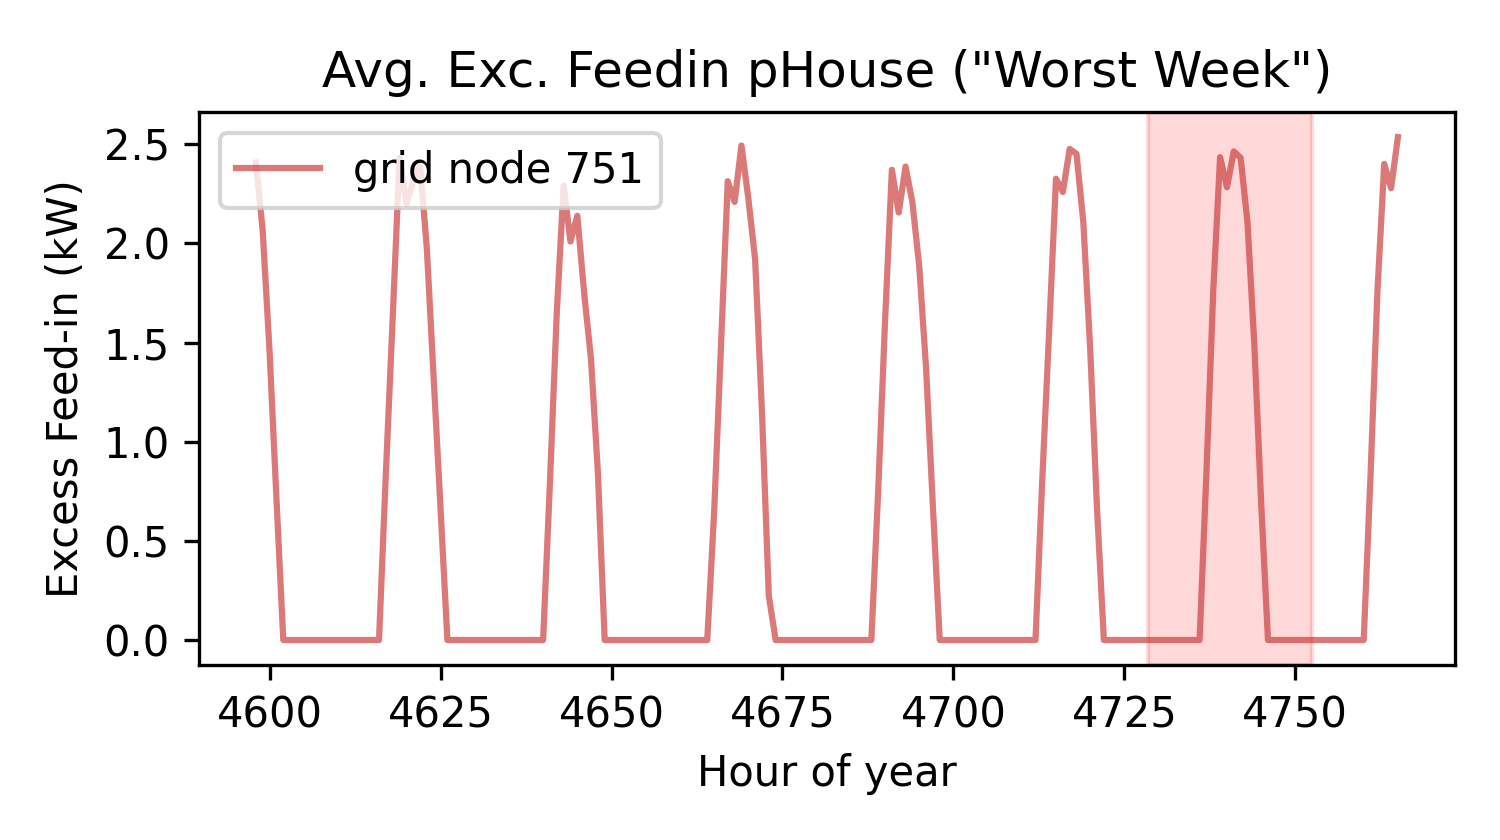
\includegraphics[width=\textwidth]{figures/worstnode_worstweek_pegid_pvalloc_LRG3_max.png}
\end{minipage}
\end{frame}

% -------------------------------------------------------
\begin{frame}{Worst Week in Worst Node}
\begin{minipage}{0.48\textwidth}
  \centering
  {\footnotesize
  \begin{tabular}{l|rrrrr}
    \toprule
    \textbf{Parameter}
      & \textbf{751}
      & \textbf{524}
      & \textbf{754}
      & \textbf{10}
      & \textbf{734} \\
    \midrule
    Peak day
      & 12.07. - 13.07.
      & 12.07. - 13.07.
      & 16.04. - 17.04.
      & 12.07. - 13.07.
      & 12.07. - 13.07. \\
    Total excess feed-in (kWh)
      & 5'970.7
      & 5'209.8
      & 3'275.0
      & 3'562.6
      & 3'063.1 \\
    n Houses
      & 379
      & 243
      & 283
      & 197
      & 167 \\
    Avg.\ excess feed-in p.\ house (kWh)
      & 15.8
      & 21.4
      & 11.6
      & 18.1
      & 18.3 \\
    Avg.\ demand p.\ house (kWh)
      & 3.0
      & 4.5
      & 6.9
      & 5.5
      & 3.3 \\
    \bottomrule
  \end{tabular}
  }
\end{minipage}\hfill
% \begin{minipage}{0.48\textwidth}
%   \centering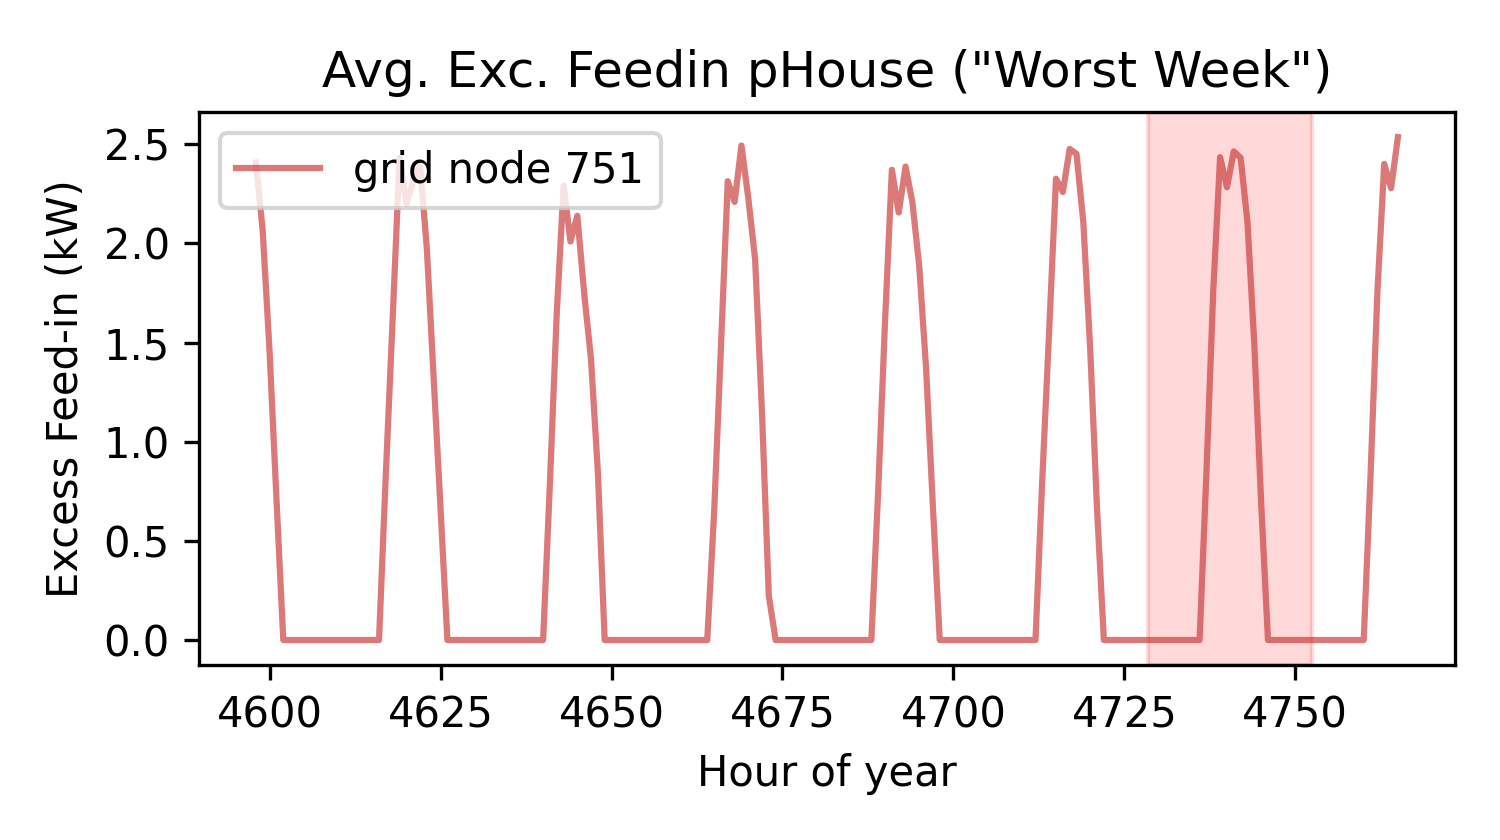
\includegraphics[width=\textwidth]{figures/worstnode_worstweek_pegid_pvalloc_LRG3_max.png}
% \end{minipage}
\end{frame}

% -------------------------------------------------------
\begin{frame}{DSO Interventions}
\begin{minipage}{0.48\textwidth}
  \centering
\includegraphics[width=\textwidth]{figures/line_PVproduction_DSOreact_excfeedin.png}
\end{minipage}\hfill
\begin{minipage}{0.48\textwidth}
  \centering
\includegraphics[width=\textwidth]{figures/line_PVproduction_DSOreact_feedin.png}
\end{minipage}
\end{frame}



%%%%%%%%%%%%%%%%%%%%%%%%%%%%%%%%%%%%%%%%%%%%%%%
\section{Outlook}

% -------------------------------------------------------
\begin{frame}{Conclusion}

  \begin{block}{Research Contribution}
    \begin{enumerate}
      \item \textbf{Problem quantification} $\rightarrow$\textit{Problems will arise in the next couple of years and might scale up fast, dependent on the growth rate of newly installed capacity.}
      \vspace{0.1cm}
      \item \textbf{Economic response} $\rightarrow$ \textit{Simple subsidy adjustments might delay grid congestion by a few years and could be even as good as a social planner's allocation.}
    \end{enumerate}
  \end{block}

  \textbf{Outlook}
  \begin{itemize}
    \item Post calculation: battery capacity for "worst week" in "worst node" (in progress).
    \item Cost comparison of subsidy spending to grid reinforcements in most affected nodes.
  \end{itemize}

  \textbf{Postponed}
  \begin{itemize}
    \item Add battery investment and battery usage to the model
    \begin{itemize}
      \item Optimized for household consumption vs.\ grid serving (quasi-obligatory for PV installations)
    \end{itemize}
  \end{itemize}

\end{frame}


%%%%%%%%%%%%%%%%%%%%%%%%%%%%%%%%%%%%%%%%%%%%%%%
\section*{Appendix}
\appendix
\backupbegin

% -------------------------------------------------------
\begin{frame}{Appendix: NPV Sensitivity - Electricity Prices}
\hypertarget{appendix_npv_hist_sensitivity}{}
\begin{minipage}{0.48\textwidth}
  \centering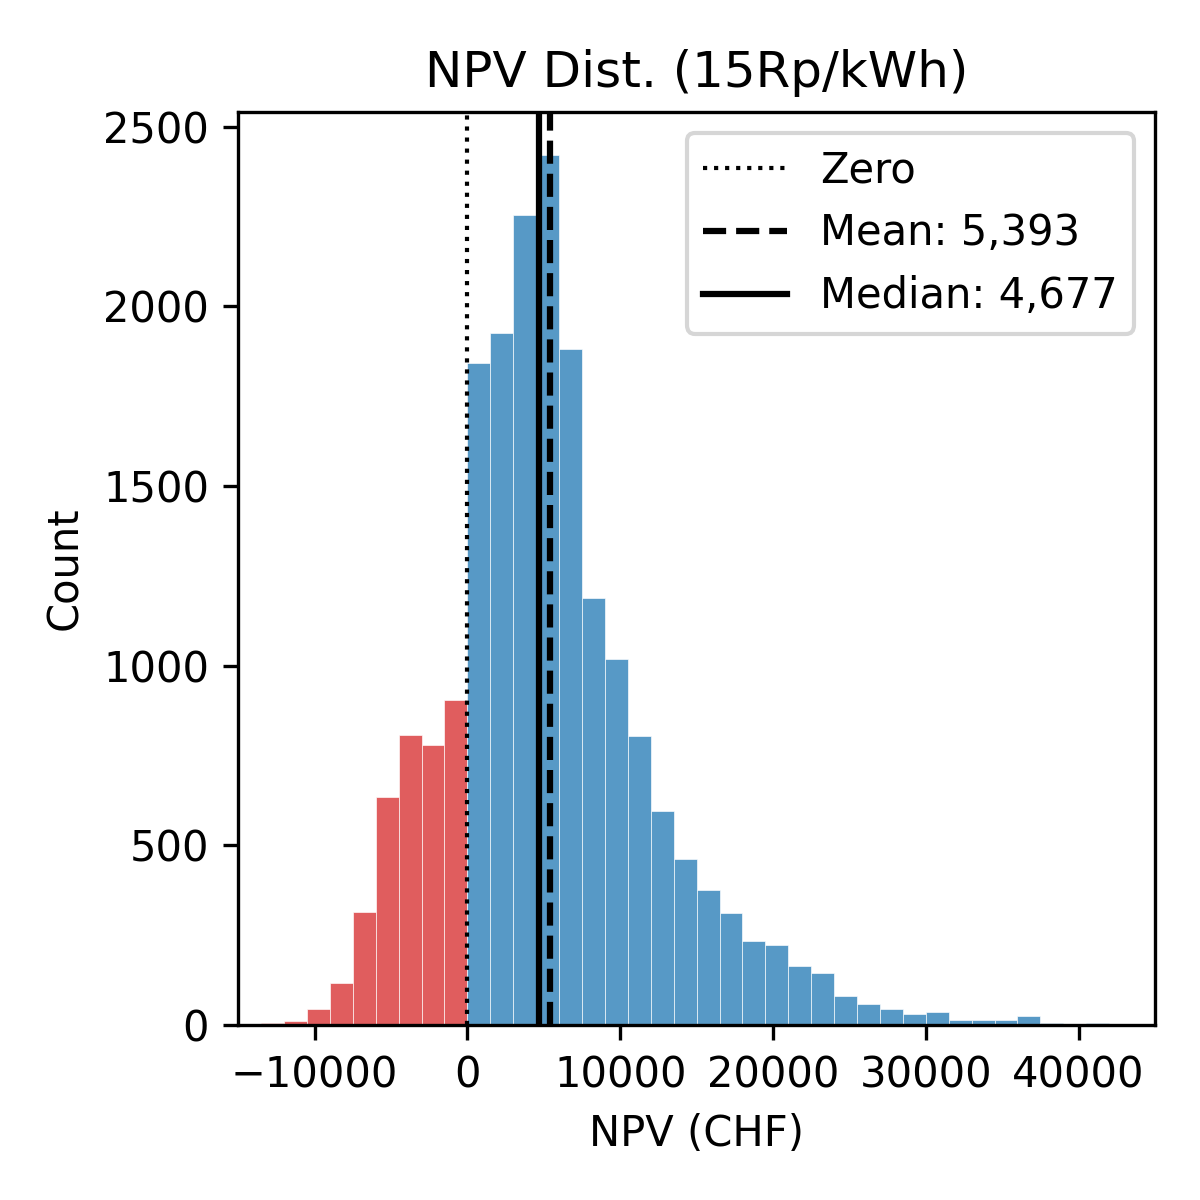
\includegraphics[width=\textwidth]{figures/NPVhist_LRG3_max_15Rp.png}
\end{minipage}\hfill
\begin{minipage}{0.48\textwidth}
  \centering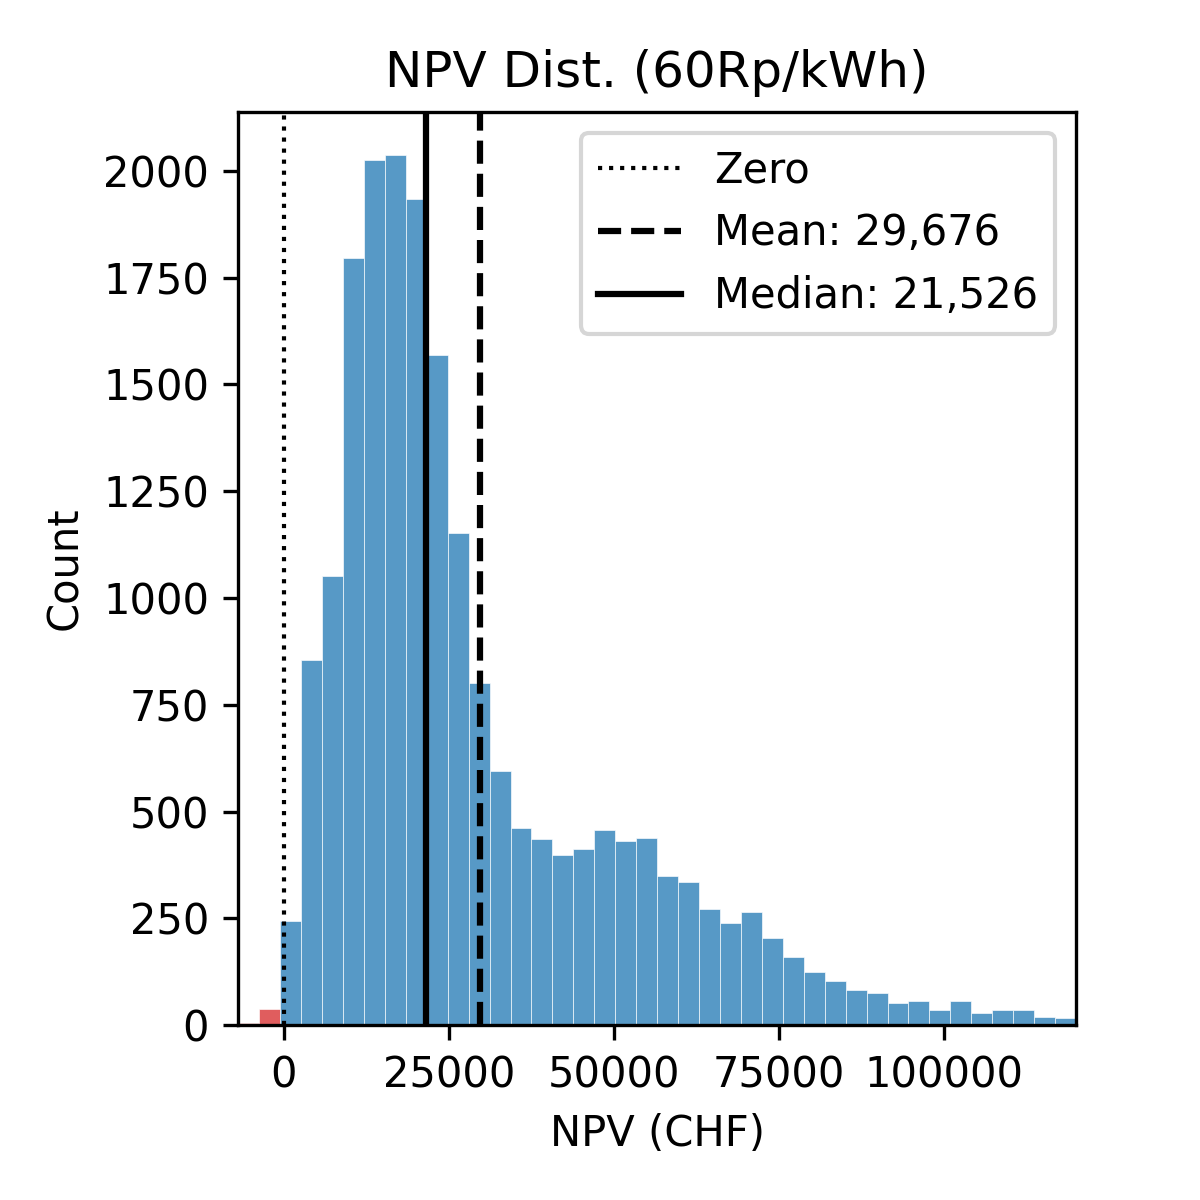
\includegraphics[width=\textwidth]{figures/NPVhist_LRG3_max_60Rp.png}
\end{minipage}
\centering
\hyperlink{mod_allocation_process}{\beamerreturnbutton{back}}
\end{frame}

% -------------------------------------------------------
\begin{frame}{Appendix: High Spatial Resolution at Large Scale}
\begin{minipage}{0.323\textwidth}
  \centering
\includegraphics[width=\textwidth]{figures/wp_topo_roof_solkat_1_3.png}
\end{minipage}\hfill
\begin{minipage}{0.323\textwidth}
  \centering
\includegraphics[width=\textwidth]{figures/wp_topo_DSO_example_1_3.png}
\end{minipage}\hfill
\begin{minipage}{0.323\textwidth}
  \centering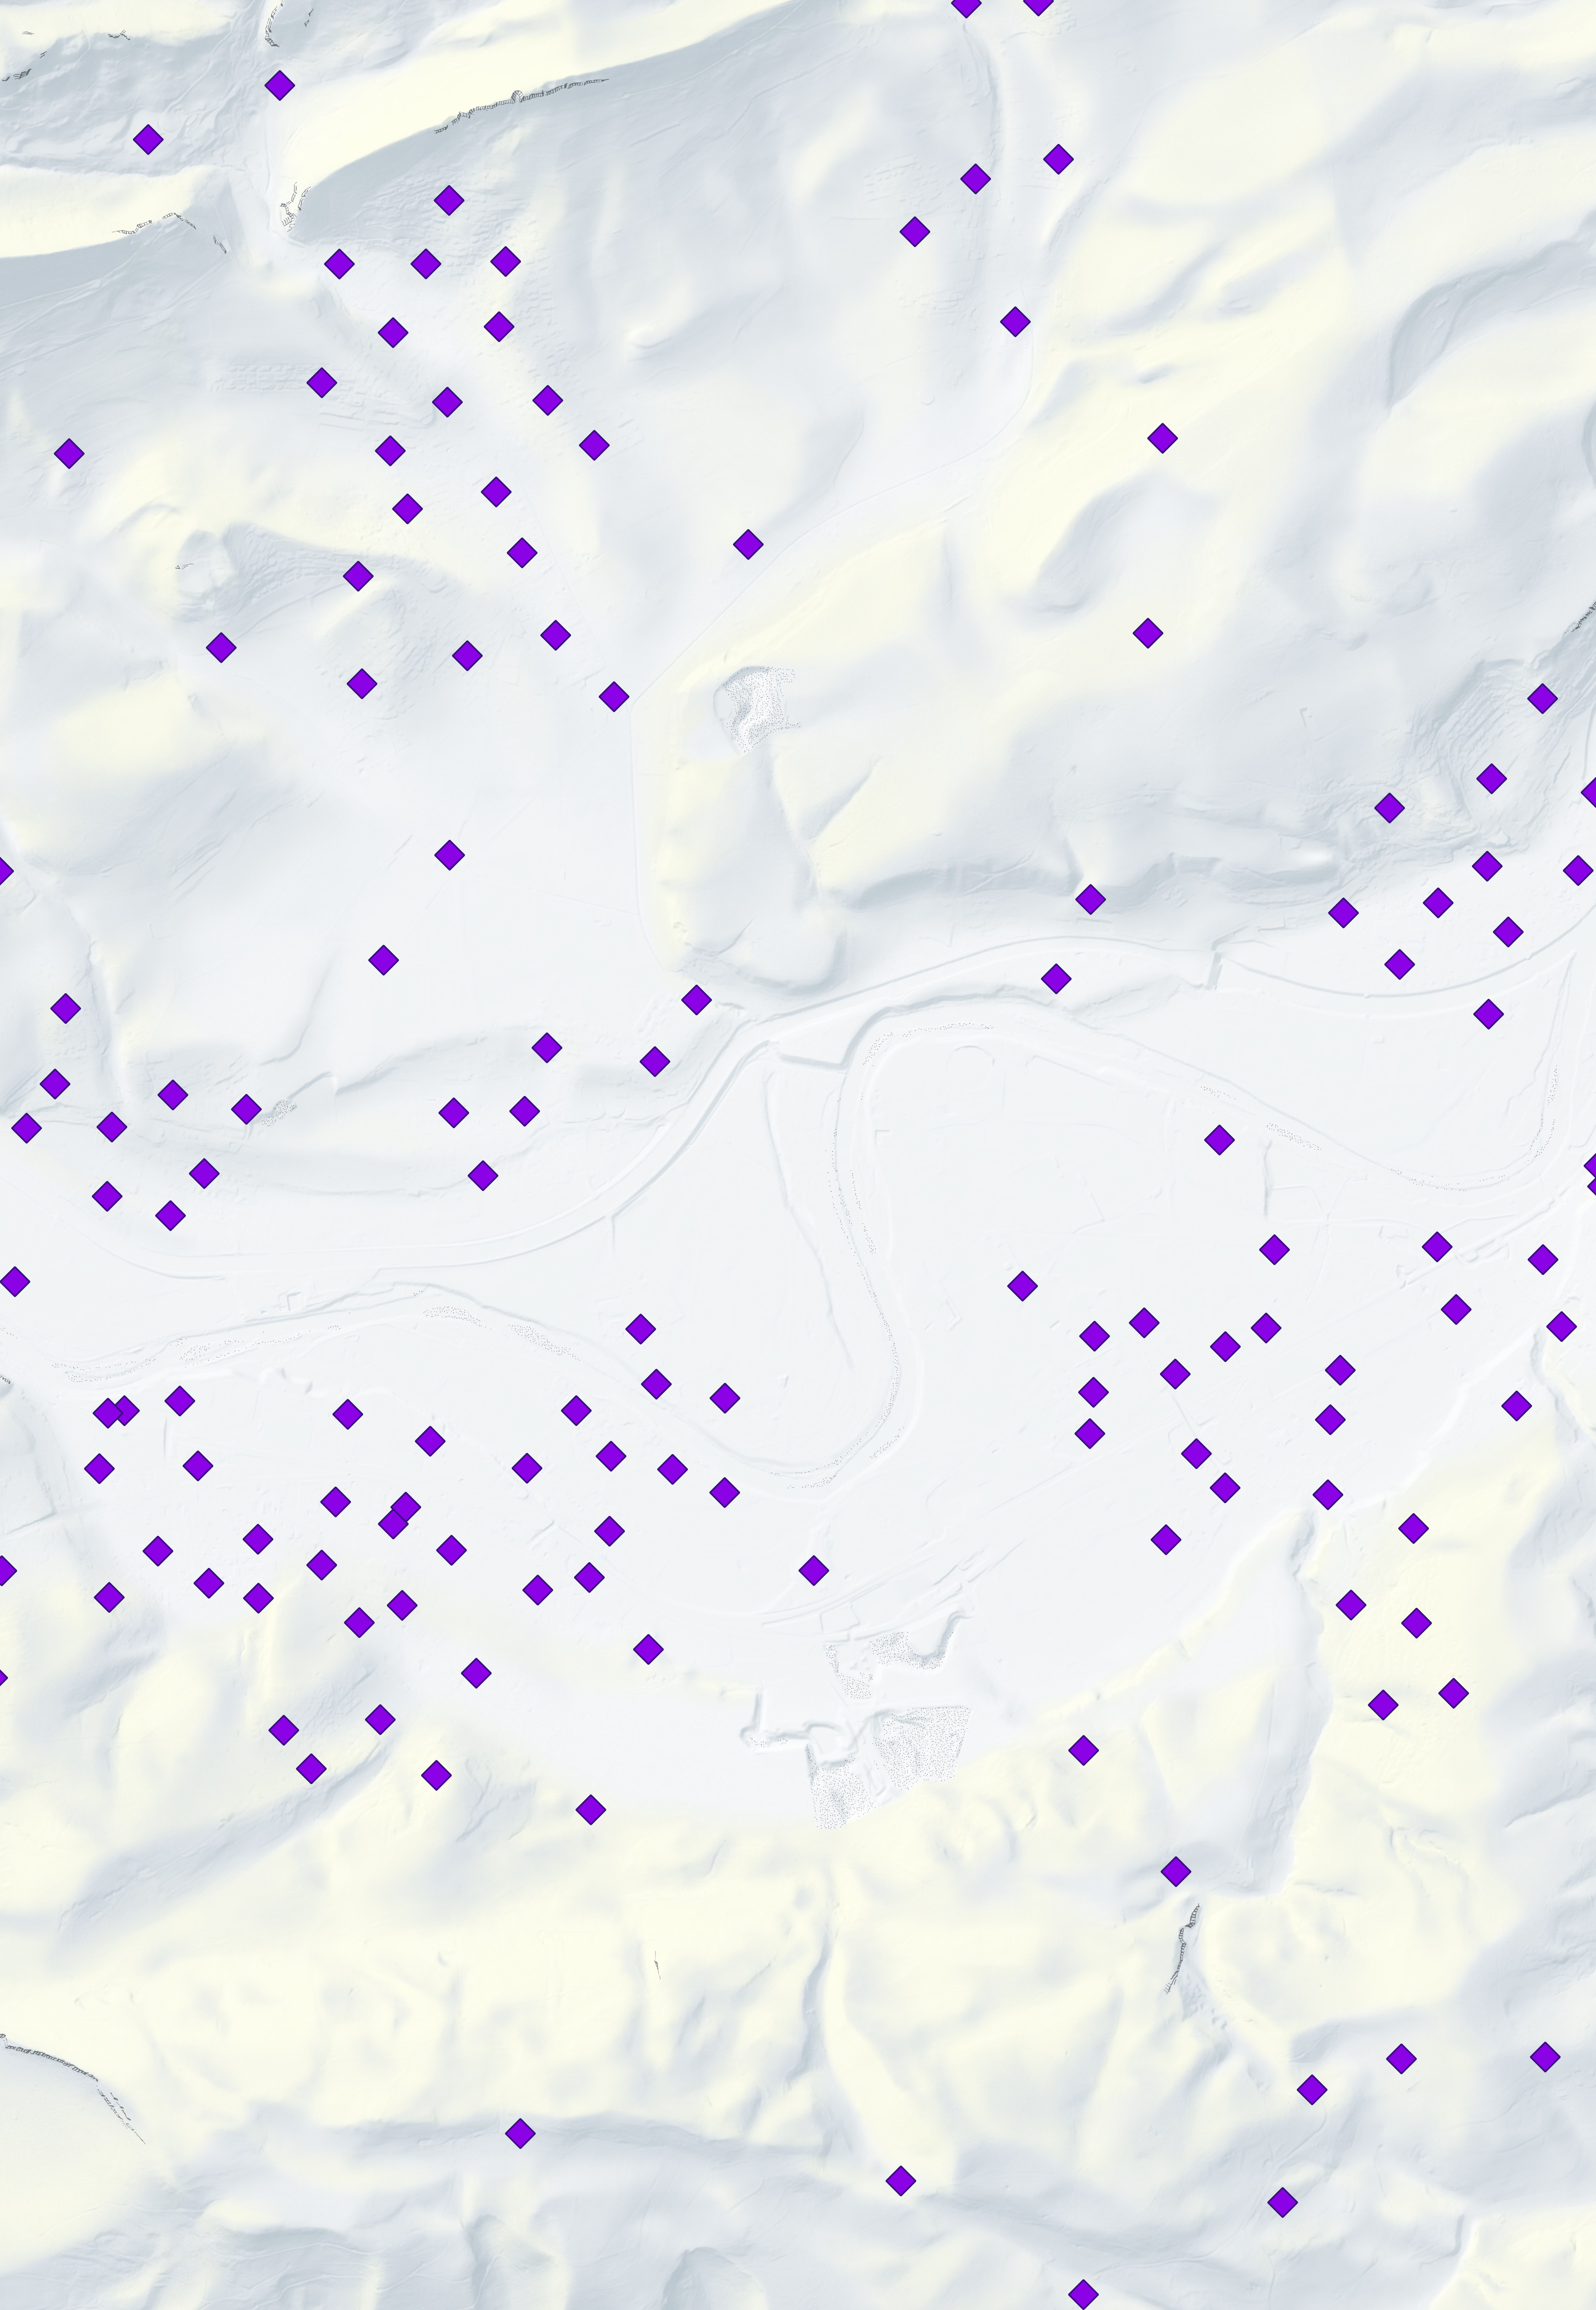
\includegraphics[width=\textwidth]{figures/wp_topo_DSO_grid_large_example_1_3.png}
\end{minipage}
\end{frame}

% -------------------------------------------------------
\begin{frame}{}
\begin{minipage}{0.479\textwidth}
  Business as Usual\\
  \centering
  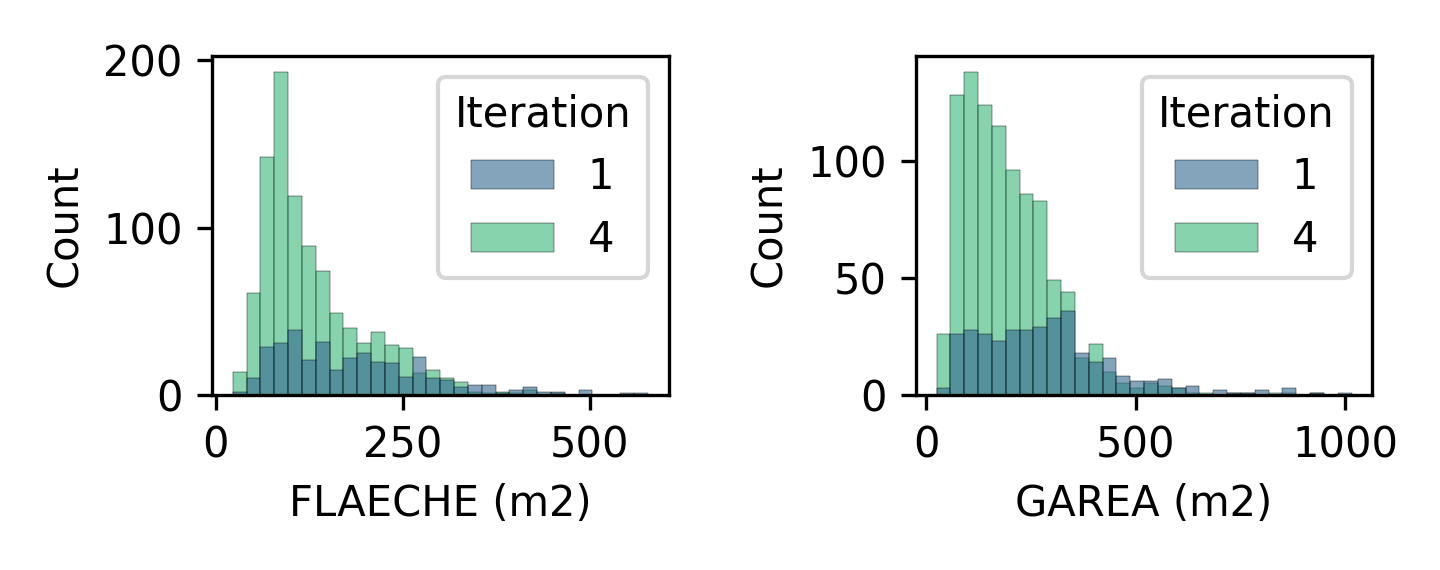
\includegraphics[width=1.0\textwidth]{figures/hist_contcharact_newinst_bu_pvalloc_LRG3_max.png}
  \vspace{-0.311cm}
  \begin{minipage}{0.49\textwidth}
    \centering\makebox[0pt][c]{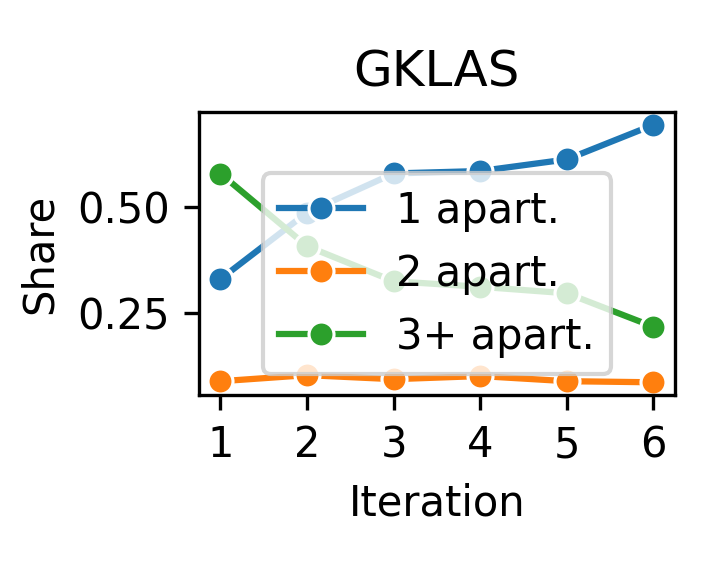
\includegraphics[width=1.05\textwidth]{figures/line_catgcharact_newinst_bu_pvalloc_LRG3_max_GKLAS.png}}
  \end{minipage}\hfill
  \begin{minipage}{0.49\textwidth}
    \centering\makebox[0pt][c]{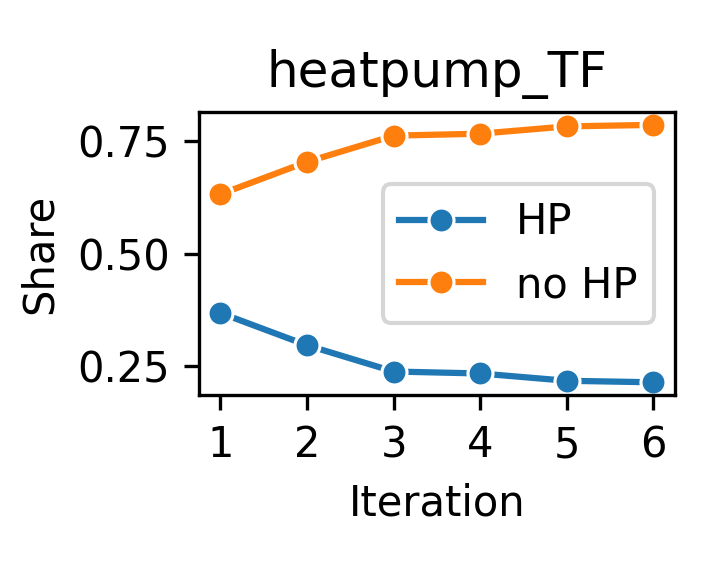
\includegraphics[width=1.05\textwidth]{figures/line_catgcharact_newinst_bu_pvalloc_LRG3_max_heatpump_TF.png}}
  \end{minipage}
  \vspace{-0.311cm}
  \begin{minipage}{0.49\textwidth}
    \centering\makebox[0pt][c]{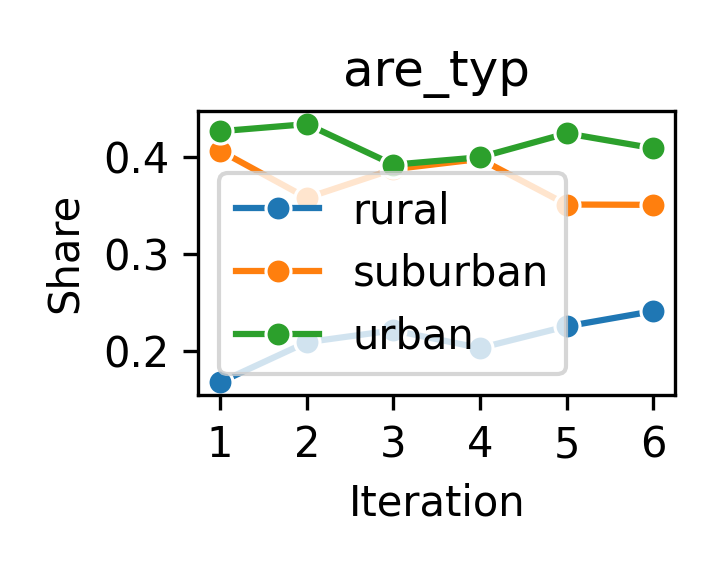
\includegraphics[width=1.05\textwidth]{figures/line_catgcharact_newinst_bu_pvalloc_LRG3_max_are_typ.png}}
  \end{minipage}\hfill
  \begin{minipage}{0.49\textwidth}
    \centering\makebox[0pt][c]{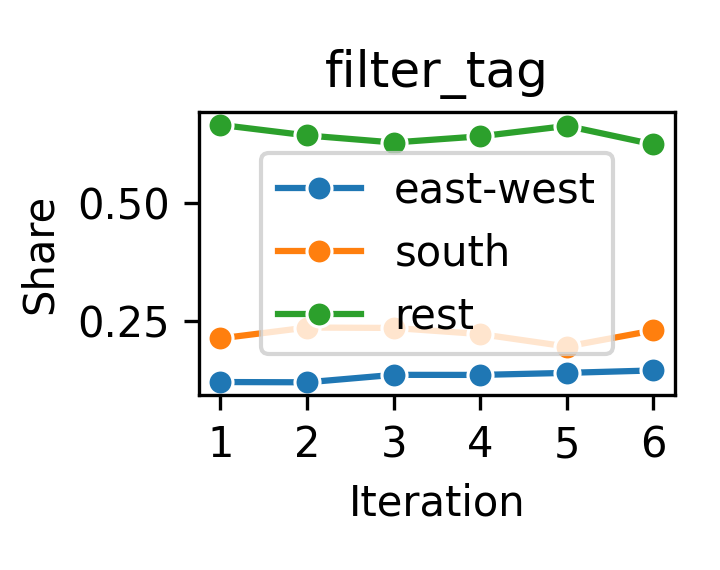
\includegraphics[width=1.05\textwidth]{figures/line_catgcharact_newinst_bu_pvalloc_LRG3_max_filter_tag.png}}
  \end{minipage}
\end{minipage}
\begin{minipage}{0.479\textwidth}
  Subsidy B\\
  \centering
  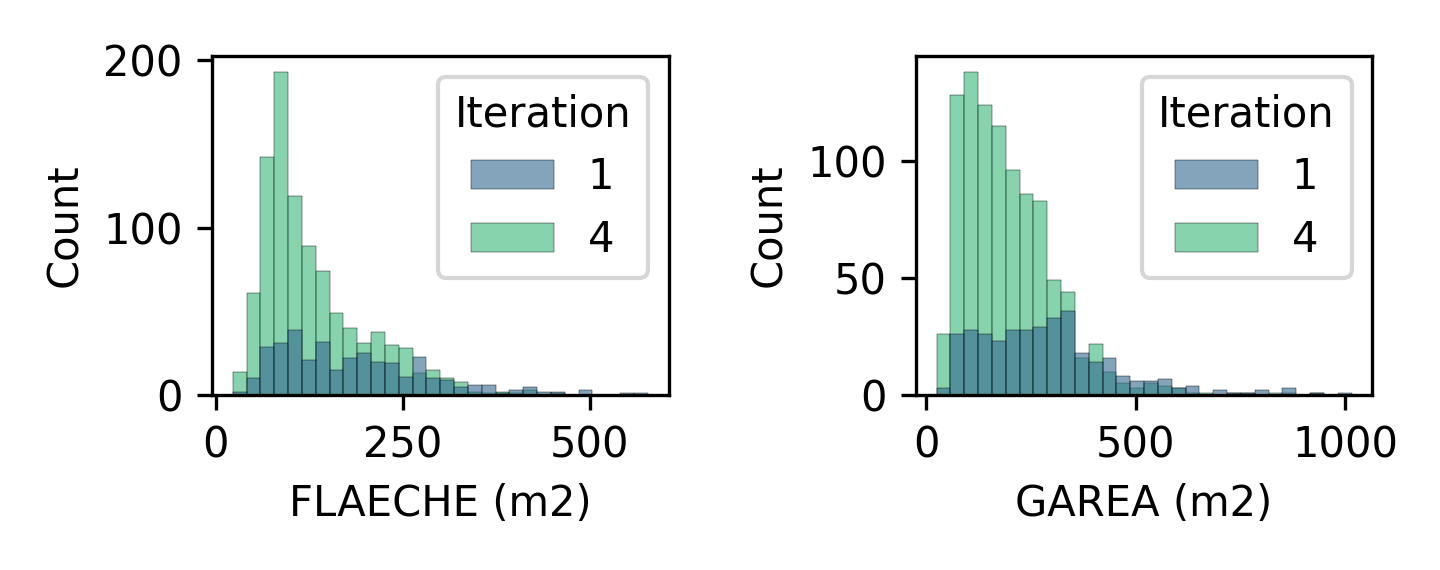
\includegraphics[width=1.0\textwidth]{figures/hist_contcharact_newinst_bu_pvalloc_LRG3_max.png}
  \vspace{-0.311cm}
  \begin{minipage}{0.49\textwidth}
    \centering\makebox[0pt][c]{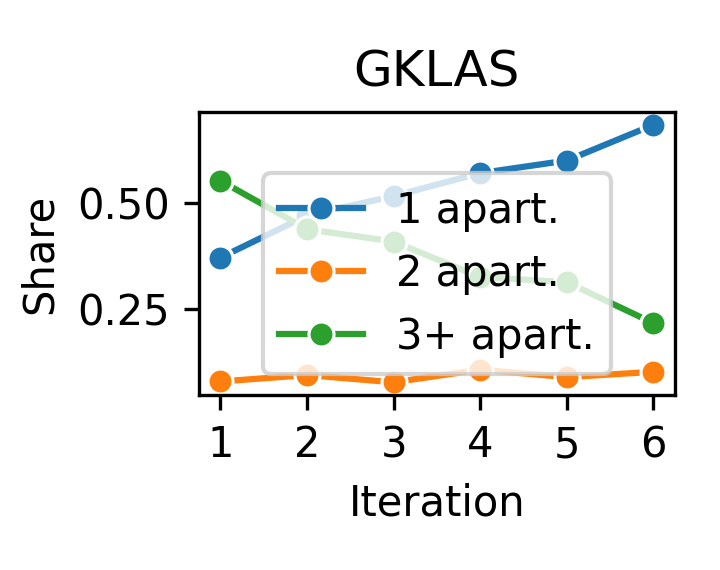
\includegraphics[width=1.05\textwidth]{figures/line_catgcharact_newinst_bu_pvalloc_LRG3_max_sBs0p8_GKLAS.png}}
  \end{minipage}\hfill
  \begin{minipage}{0.49\textwidth}
    \centering\makebox[0pt][c]{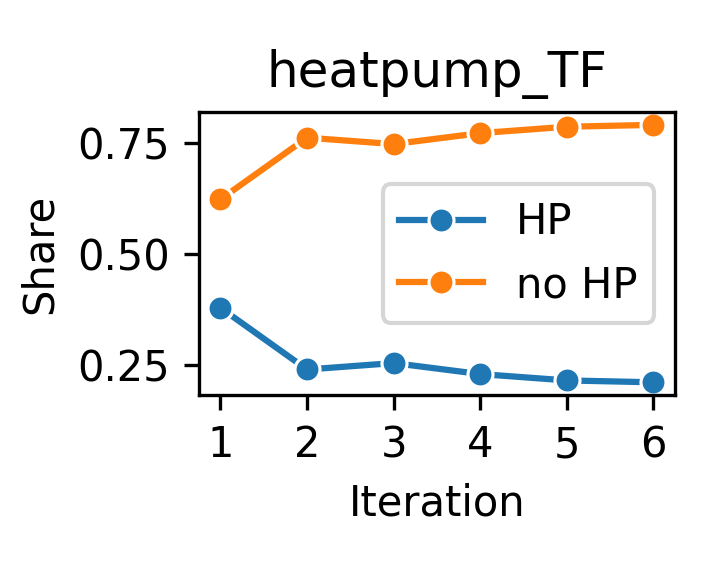
\includegraphics[width=1.05\textwidth]{figures/line_catgcharact_newinst_bu_pvalloc_LRG3_max_sBs0p8_heatpump_TF.png}}
  \end{minipage}
  \vspace{-0.311cm}
  \begin{minipage}{0.49\textwidth}
    \centering\makebox[0pt][c]{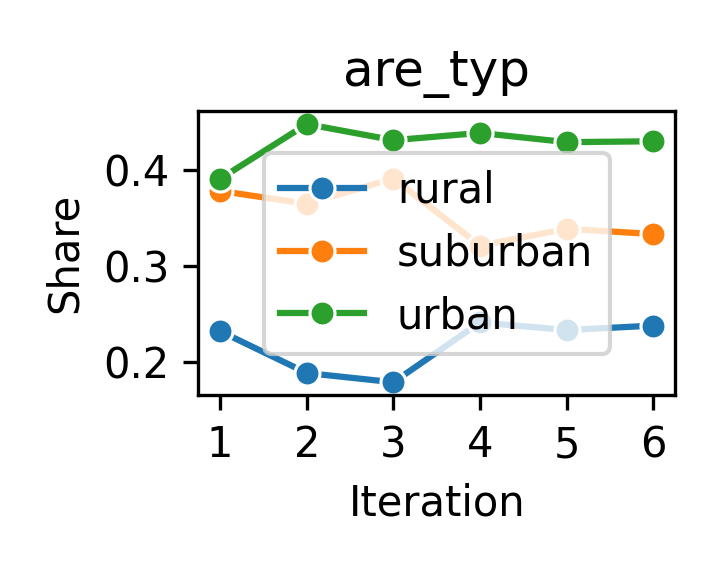
\includegraphics[width=1.05\textwidth]{figures/line_catgcharact_newinst_bu_pvalloc_LRG3_max_sBs0p8_are_typ.png}}
  \end{minipage}\hfill
  \begin{minipage}{0.49\textwidth}
    \centering\makebox[0pt][c]{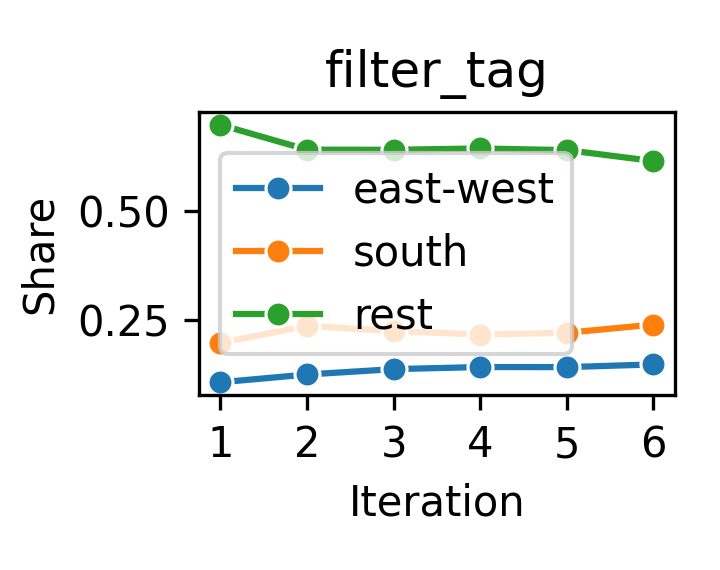
\includegraphics[width=1.05\textwidth]{figures/line_catgcharact_newinst_bu_pvalloc_LRG3_max_sBs0p8_filter_tag.png}}
  \end{minipage}
\end{minipage}
\end{frame}

% -------------------------------------------------------
\begin{frame}{Appendix: Model Grid Analysis EP2050+}
\hypertarget{appendix_model_grid_analysis}{}
\vspace{-\baselineskip}
\begin{figure}
  \centering
  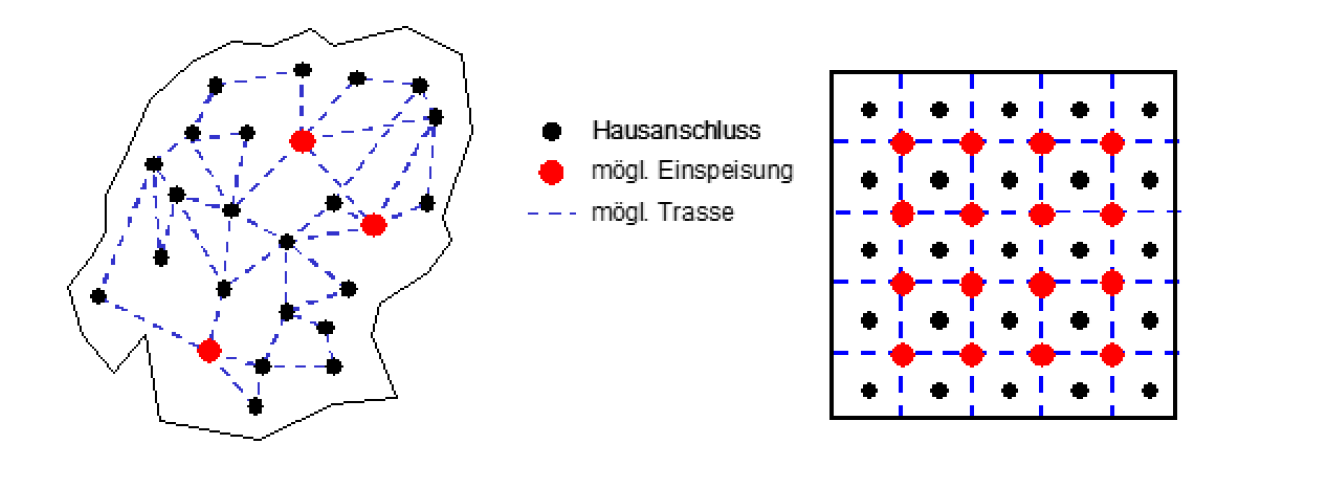
\includegraphics[width=0.8\textwidth]{figures/bfe_ep2050_netz_MNA_notitle.PNG}
\end{figure}
\vspace{-\baselineskip}
\small\centering
\textit{Comparison between the real (left) and homogeneous model assumed grid topology \cite{bfe_ep2050_netz2022}}
\hyperlink{back}{\beamerreturnbutton{Literature}}
\end{frame}

% -------------------------------------------------------
\begin{frame}{Appendix: Calibrated Random Forest}
\hypertarget{appendix_randomforest_scatterplot}{}
\vspace{-\baselineskip}
\begin{figure}
  \centering
  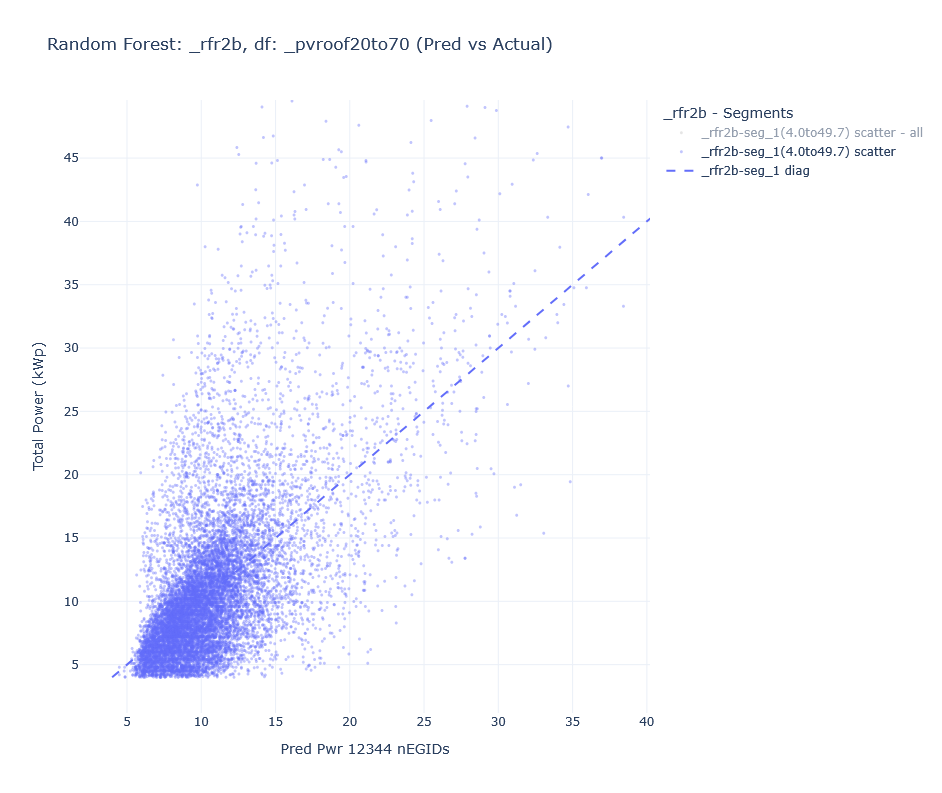
\includegraphics[width=0.56\textwidth]{figures/calib_rfr2_predvsactual.png}
\end{figure}
\vspace{-\baselineskip}
\small\centering
\textit{Scatterplot for actual and predicted installation sizes (incl.\ 45° diagonal) of calibrated random forest regression on 61270 Swiss houses with a PV installation, between 20 to 70 percent of available roof partition used.}
\hyperlink{mod_structure_agents}{\beamerreturnbutton{back}}
\end{frame}

% -------------------------------------------------------
\begin{frame}{Appendix: Interpolated Cost Function}
\hypertarget{appendix_cost_function}{}
\vspace{-\baselineskip}
\begin{figure}
  \centering
  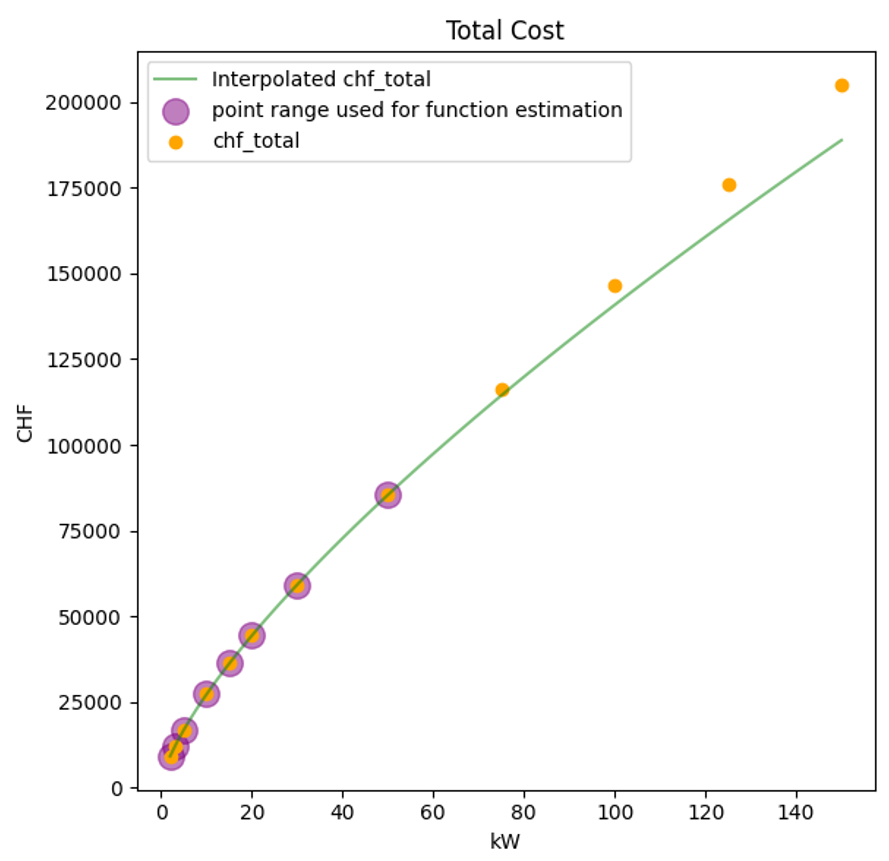
\includegraphics[width=0.56\textwidth]{figures/pvinstcost_table.png}
\end{figure}
\vspace{-\baselineskip}
\small\centering
\textit{Interpolation approximation function (green, only on small scale installations) based on cost assumptions in the technical model appendix of energieschweiz.}
\hyperlink{mod_structure_agents}{\beamerreturnbutton{back}}
\end{frame}

% -------------------------------------------------------
\begin{frame}{Appendix: RES Targets 2050 Switzerland}
\hypertarget{appendix_res_targets}{}
\vspace{-\baselineskip}
\begin{figure}
  \centering
  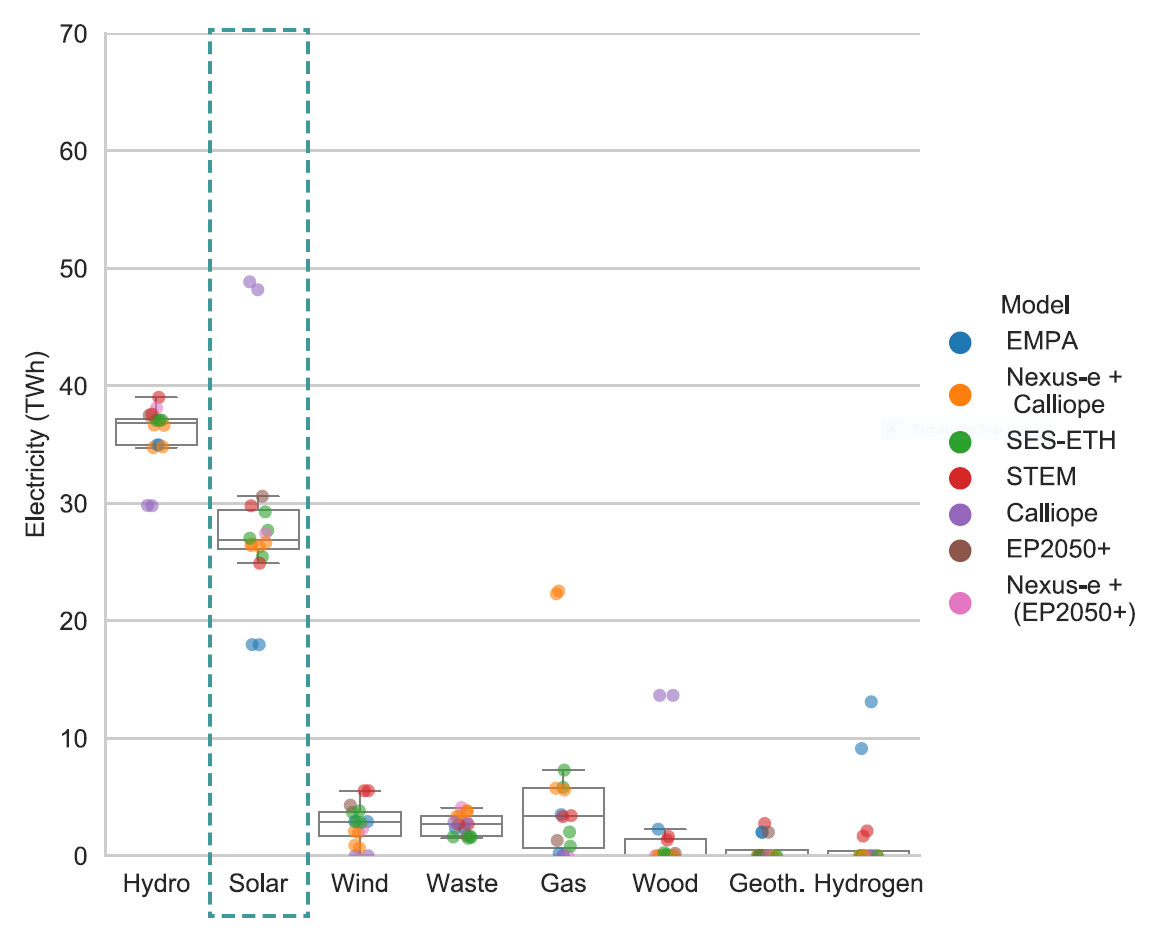
\includegraphics[width=0.56\textwidth]{figures/eth_summerschool_scenario_agg_notitle.png}
\end{figure}
\vspace{-\baselineskip}
\hyperlink{motivation_relevance}{\beamerreturnbutton{back}}
\end{frame}


%%%%%%%%%%%%%%%%%%%%%%%%%%%%%%%%%%%%%%%%%%%%%%%
\renewcommand{\bibfont}{\footnotesize}
\begin{frame}[allowframebreaks]{References}
  \printbibliography
\end{frame}

\end{document}
